% VLDB template version of 2020-08-03 enhances the ACM template, version 1.7.0:
% https://www.acm.org/publications/proceedings-template
% The ACM Latex guide provides further information about the ACM template

\documentclass[sigconf, nonacm]{acmart}

%% The following content must be adapted for the final version
% paper-specific
\newcommand\vldbdoi{XX.XX/XXX.XX}
\newcommand\vldbpages{XXX-XXX}
% issue-specific
\newcommand\vldbvolume{14}
\newcommand\vldbissue{1}
\newcommand\vldbyear{2020}
% should be fine as it is
\newcommand\vldbauthors{\authors}
\newcommand\vldbtitle{\shorttitle} 
% leave empty if no availability url should be set
\newcommand\vldbavailabilityurl{URL_TO_YOUR_ARTIFACTS}
% whether page numbers should be shown or not, use 'plain' for review versions, 'empty' for camera ready
\newcommand\vldbpagestyle{plain} 
\usepackage{amsmath}
\usepackage{graphicx}
\usepackage{subfig}
\usepackage{caption}
\usepackage{subcaption}

\begin{document}
\title{DH2323 Computer Graphics and Interaction \\ Recursive Backwards Ray Tracing \\ Project Report}

%%
%% The "author" command and its associated commands are used to define the authors and their affiliations.
\author{Ramona Häuselmann}
\affiliation{%
  \institution{KTH Royal Institute of Technology}
}
\email{ramonaha@kth.se}



%%
%% The abstract is a short summary of the work to be presented in the
%% article.
\begin{abstract}
We present the implementation of a simple recursive backwards ray tracing algorithm based on the algorithm introduced by John Turner Whitted in 1980.
In the scope of the project we explore details and improvements of a basic ray tracing algorithm to explore its capabilities and limitations.

The system is capable of rendering triangles and spheres with glossy, diffuse, specular and transmissive as well as textured materials. It uses a
bounding volume hierarchy for increased performance, sub sampling to reduce aliasing effects and an area lighting model for soft shadows.
\begin{figure}[h]
  \centering
  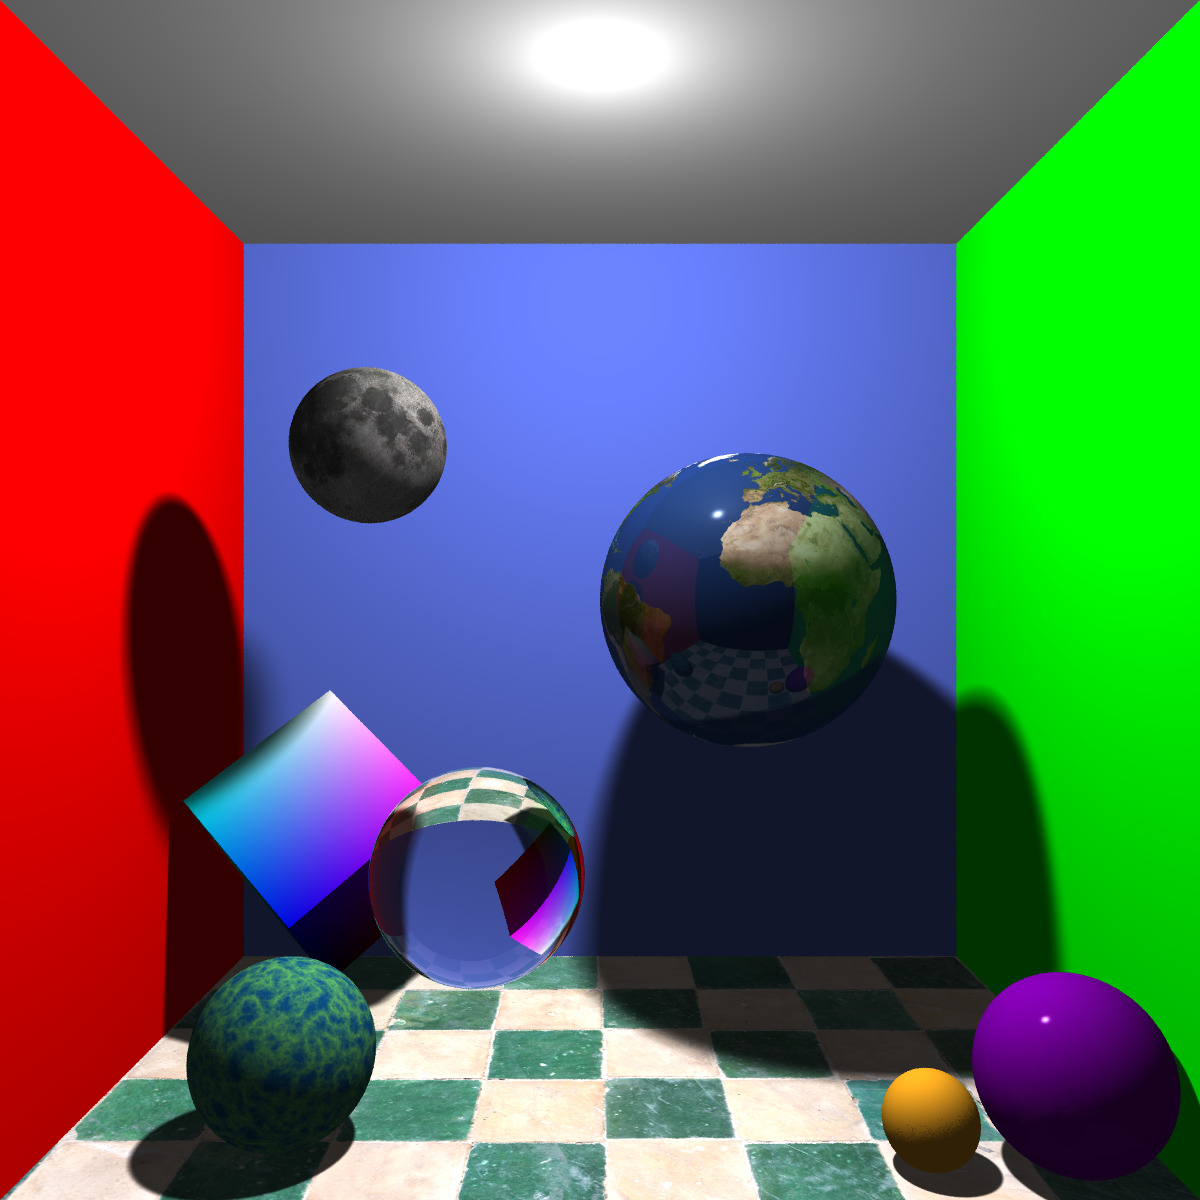
\includegraphics[width=\linewidth]{figures/cornell_showcase.jpg}
  \caption{Cornell box scene. Rendered with 4 super samples per pixel and a rectangle area light for soft shadows.}
  \label{fig:cornell}
\end{figure}

Figure 1 shows the final result. The scene consists of a glossy, specular sphere with earth map texture, a diffuse sphere with moon texture,
a diffuse cube with rainbow texture, a glass sphere, a purple, specular sphere, a yellow, diffuse sphere and a diffuse sphere with procedural texture (green and blue)
\end{abstract}
\maketitle



%%% do not modify the following VLDB block %%
%%% VLDB block start %%%
\ifdefempty{\vldbavailabilityurl}{}{
% \vspace{.3cm}
\begingroup\small\noindent\raggedright\textbf{Source Code:}\\
The source code and data can be found at\\ \url{https://github.com/rhaeus/basic_raytracer}.
\endgroup
}
%%% VLDB block end %%%

\section{Introduction}
In the field of computer graphics there are many different techniques for generating realistic looking images. In this project we explore
one early approach to solving the rendering equation. It was introduced by John Turner Whitted in 1980. We based our implementation on this idea and 
added several improvements.\\
The implemented raytracer is a so called backwards raytracer. In nature light is emitted from every light source and bounces infinitely on objects until
it finally reaches our eye. Given that most of the rays never reach our eye it would be wasteful and simply computationally not feasible to trace each ray
starting from the light source. A backwards raytracer follows the inverse approach: It follows the rays backwards, starting from the eye into the scene.
This reduces the computational complexity but also has the disadvantage of missing global lighting effects since only rays that finally reach the eye
are considered in the calculations. There are many approaches that take global lighting into account, e.g. Photon Mapping, Path Tracing or Radiosity. 
In this project we want to explore the basic techniques to build a foundation for further work.

\section{General Algorithm}
The raytracer calculates a primary ray for each image pixel starting at the camera position. It then calculates if the ray intersects any of the objects in the scene.
If an intersection occurs, the algorithm calculates the color at this position, depending on the object material by using the Phong illumination model.
For shadow calculation the raytracer casts a shadow ray to each light source to check if the surface point receives direct lighting.
If the surface of the intersected object is reflective and/or refractive the raytracer calculates the reflection and refraction rays using Snell's law as well
as the amount of reflection and refraction based on the material properties by using the Fresnel equations. This process is repeated recursively until the 
ray hits a diffuse surface without reflection or refraction, misses the scene or the max recursion depth is reached.

\clearpage

\section{Lighting and color calculation}
For illumination and coloring we use the Phong illumination model. The color of an object surface is calculated as

\begin{equation}
  \begin{split}
      color &= ambientColor \\
      &+ diffuseAndSpecularColor \\
      &+ reflectiveAndRefractiveColor
  \end{split}
\end{equation}
We use an ambient color term to simulate global illumination. This term adds a small constant illumination so that surfaces without direct lighting are not pitch black.
It is calculated as . The resulting diffuse and specular color is calculated by
\[ambientColor=surfaceColor*0.2\]
\[diffuseColor=surfaceColor*lightColor*\langle N,L \rangle\] 
where N is the surface normal and L is the light incidence direction. 
\[specularColor=lightColor* \langle R, V \rangle^p\]
where R is the direction of light reflection, V is the viewing direction and p represents
the shininess of the surface.\\
The surface color, N and p are determined by the object and its material.
The reflective and refractive color components are calculated by casting rays in reflection and refraction direction.


\section{Texture Mapping}
The system supports three different ways of texturing:
\begin{itemize}
  \item texture color mapping using a texture file
  \item procedural texture color generation using Perlin noise
  \item procedural normal generation using Perlin noise
\end{itemize}

\subsection{UV Mapping}
\textbf{Sphere texture mapping} 
To texture a spherical object we map the 3D surface coordinate to a 2D texture coordinate using the following equation.
\[u=0.5+\frac{\arctan(d_x, d_z)}{2\pi}\]
\[v=0.5-\frac{\arcsin(d_y)}{\pi}\]
We use those coordinates to lookup the color value in the color map file.\\
\\
\textbf{Triangle texture mapping} 
To map a 2D texture to a 3D triangle we need to interpolate between the vertices. For interpolation we use barycentric coordinates.
Let \(v_0, v_1, v_2\) be the vertices of the triangle and \(pos\) the 3D position of which we want to calculate the color value. 
\(t_0, t_1, t_2\) are the 2D texture coordinates of each vertex.
We first express \(pos\)  in terms of \(v_0, v_1, v_2\):
\[pos=\alpha*v_0 + \beta*v_1 + \gamma*v_2\]
Then we can use those coefficients for interpolating between the vertex texture coordinates to obtain the 2D texture coordinate \(tex\) as
\[tex=\alpha*t_0 + \beta*t_1 + \gamma*t_2\]

\subsection{Procedural texture generation}

\subsection{Procedural normal mapping}

\section{Improvements}

\subsection{Bounding Volume Hierarchy (BVH)}
The speed of the ray tracing algorithm is limited by the performance of the ray-primitive intersection tests. In order to calculate the scene, the algorithm
must perform an intersection test for each ray with each primitive (triangle, sphere) in the scene. 
In a naive approach for each ray we could simply iterate over all primitives. This results in a lot of unnecessary intersection tests because 
most rays only intersect with a few primitives. \\
To improve performance we use a \textbf{B}ounding \textbf{V}olume \textbf{H}ierarchy data structure. This data structure hierarchically divides the space
into smaller sub spaces, represented by an axis-aligned bounding box (AABB). Each primitive is stored in the corresponding container. The root container of this 
tree represents the entire scene space. To perform intersection tests we recursively check intersections with the AABB of the sub spaces and only descend further
if this bounding box is hit by a ray. This way we can early discard a lot of intersection tests with the primitives stored in the sub space if the bounding volume is
not hit by the ray.\\
We are using a BVH with a max depth of 16. Each space can be divided into 8 sub spaces and we allow for a maximum of 4 primitives in each space before it is split up.
The achieved speed up is shown below. We rendered the scene shown in Figure 1 with and without the use of the BVH.
The scene consists of 27 primitives and was rendered with a resolution of 1200x1200 pixels. We use 4 sub samples per pixel and 100 samples for the area light.
A total of 6637052 rays were cast.

\begin{table}[h]
  \caption{BVH Performance}
  \label{tab:bvhperformance}
  \begin{tabular}{lrr}
    \toprule
     & Without BVH & With BVH \\
    \midrule
    ray triangle tests & 13,264,817,544& 1,835,448,170 \\
    ray triangle hits  & 565,645,299 & 565,645,281\\
    ray sphere tests & 3,617,677,512 & 1,240,731,817\\
    ray sphere hits & 97,583,742 & 97,583,742\\
    AABB tests & - & 9,037,706,495\\
    abort early (AABB miss) & - & 6,296,976,881\\
    render time & 540s & 286s\\
    \bottomrule
  \end{tabular}
\end{table}




\subsection{Soft shadows (area light)}
When lighting a scene the simplest approach is to use a point light source, meaning the light is emitted at a singular point in space. This is
of course not very realistic since every light source in the real world has some expansion. Point light sources lead to very sharp shadows as seen in 
Figure \ref{fig:lightSampling} a).
and are not very realistic. To render softer shadows we can simulate a light source that has extents. In this project we used a rectangle light source.
Instead of sampling a single point for the lighting calculation for an area light we would now have to integrate over the entire light source area.
Since this is very computationally intensive we can use Monte Carlo integration to solve the problem:\\
We can approximate the light intensity at every point in the scene by sampling N points on the light source area. We then calculate if this 
point casts a shadow on the current scene point. Every sample point is weighted by 1/N. The final color of the scene point is then given by
\[ resultingColor = color * lightIntensity \] 
where \(color\) is calculated using the Phong illumination model and 
\[lightIntensity = \frac{\#notShadowingSamplePoints}{N}\]
The pattern in which we choose to sample the points on the light source impact the look of the shadows. We studied two approaches:
\begin{itemize}
  \item Uniform grid: divide the area of the light source with a uniform grid and sample a point at the center of each grid cell. 
  This leads to a visible pattern in the shadow as shown in Figure \ref{fig:lightSampling} b).
  \item Jittered grid: divide the area of the light source with a uniform grid but instead of sampling at the center we choose the position randomly.
  This eliminates the pattern but also leads to a noisier result as shown in Figure \ref{fig:lightSampling} c). By increasing the number of samples
  the noise can be reduced and a smooth shadow is obtained (Figure \ref{fig:lightSampling} d))

\end{itemize}
% \begin{figure*}
%   \centering
%   \begin{subfigure}[b]{0.3\textwidth}
%       \centering
%       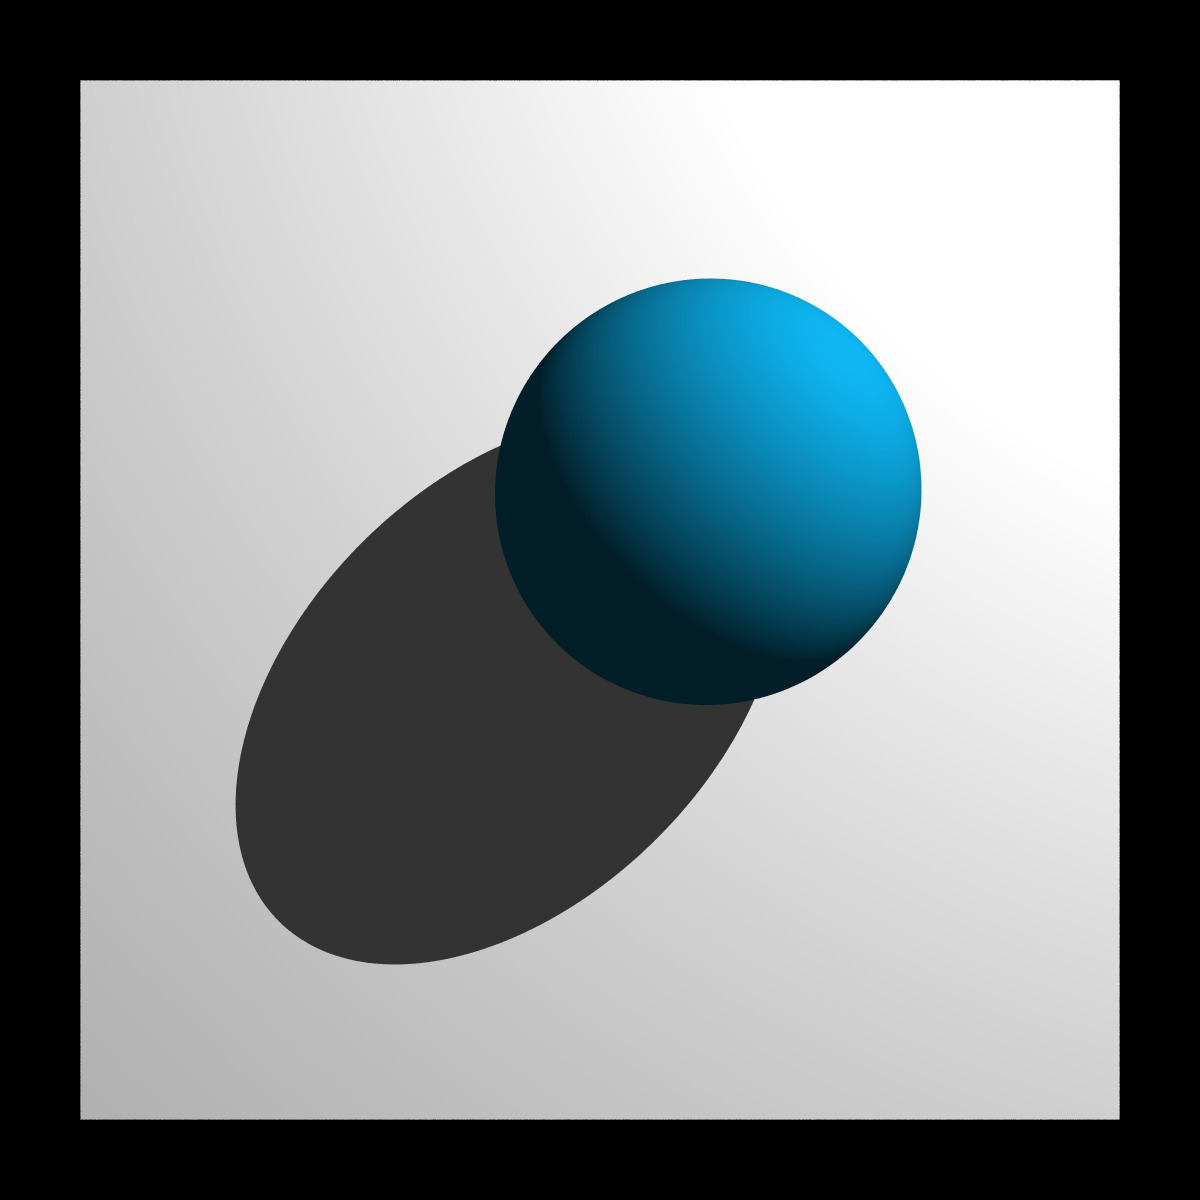
\includegraphics[width=4cm]{figures/shadow/shadow_pointlight.jpg}
%       \caption{$y=x$}
%       \label{fig:y equals x}
%   \end{subfigure}
%   \hfill
%   \begin{subfigure}[b]{0.3\textwidth}
%       \centering
%       \includegraphics[width=\textwidth]{graph2}
%       \caption{$y=3sinx$}
%       \label{fig:three sin x}
%   \end{subfigure}
%   \hfill
%   \begin{subfigure}[b]{0.3\textwidth}
%       \centering
%       \includegraphics[width=\textwidth]{graph3}
%       \caption{$y=5/x$}
%       \label{fig:five over x}
%   \end{subfigure}
%      \caption{Three simple graphs}
%      \label{fig:three graphs}
% \end{figure}

% \FloatBarrier
\begin{figure}[ht]
  \centering
  \subfloat[Sharp shadow due to point light]{
    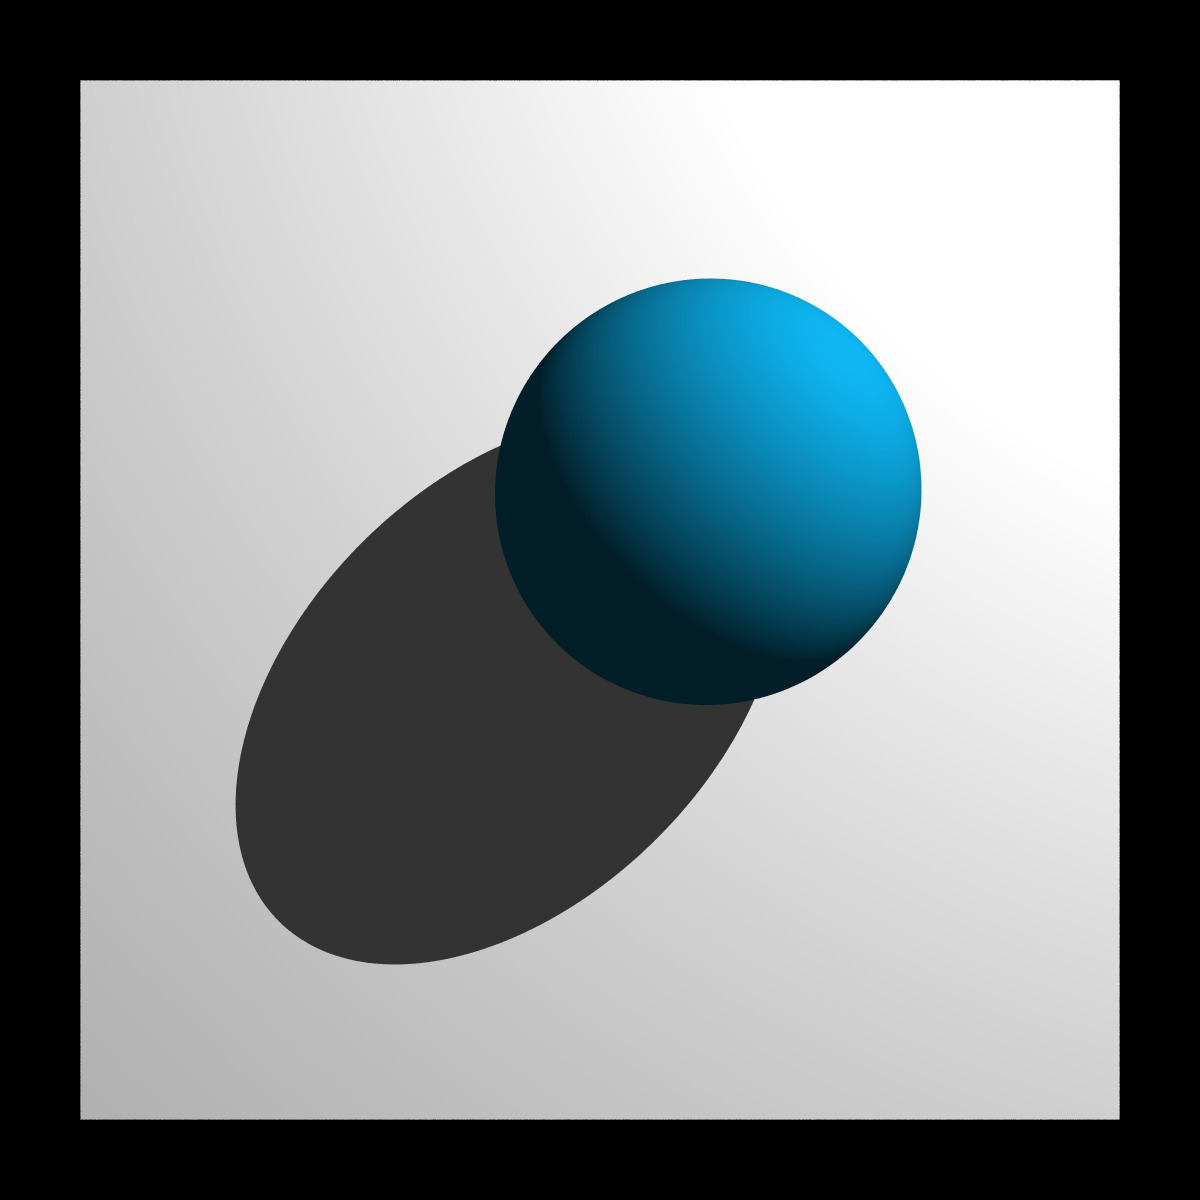
\includegraphics[width=4cm]{figures/shadow/shadow_pointlight.jpg}
    % \caption{Sharp shadow due to point light}
    % \label{fig:shadowPointLight}
  }
  \subfloat[Pattern in shadow.\\ Area light with 4 uniformly selected sample points]{
    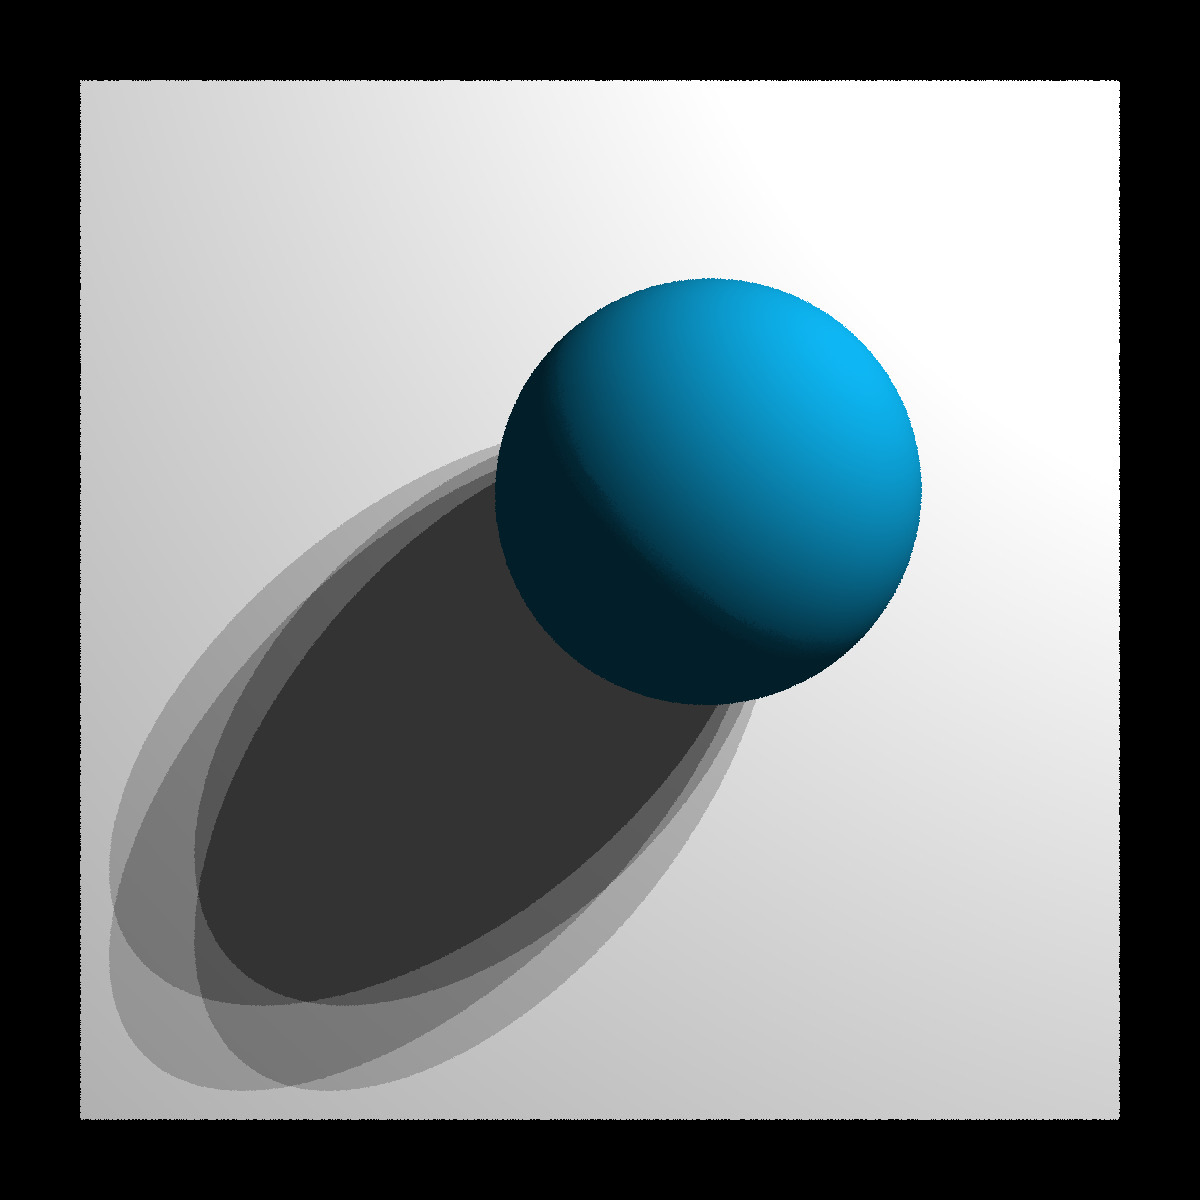
\includegraphics[width=4cm]{figures/shadow/shadow_rectangle_4_uniform.jpg}
    % \caption{Pattern in shadow. Area light with 4 uniformly selected sample points}
    % \label{fig:shadowAreaLight4uniform}
  }
  \hspace{0mm}
  \subfloat[Softer but noisy shadow.\\Area light with 4 randomly selected sample points]{
    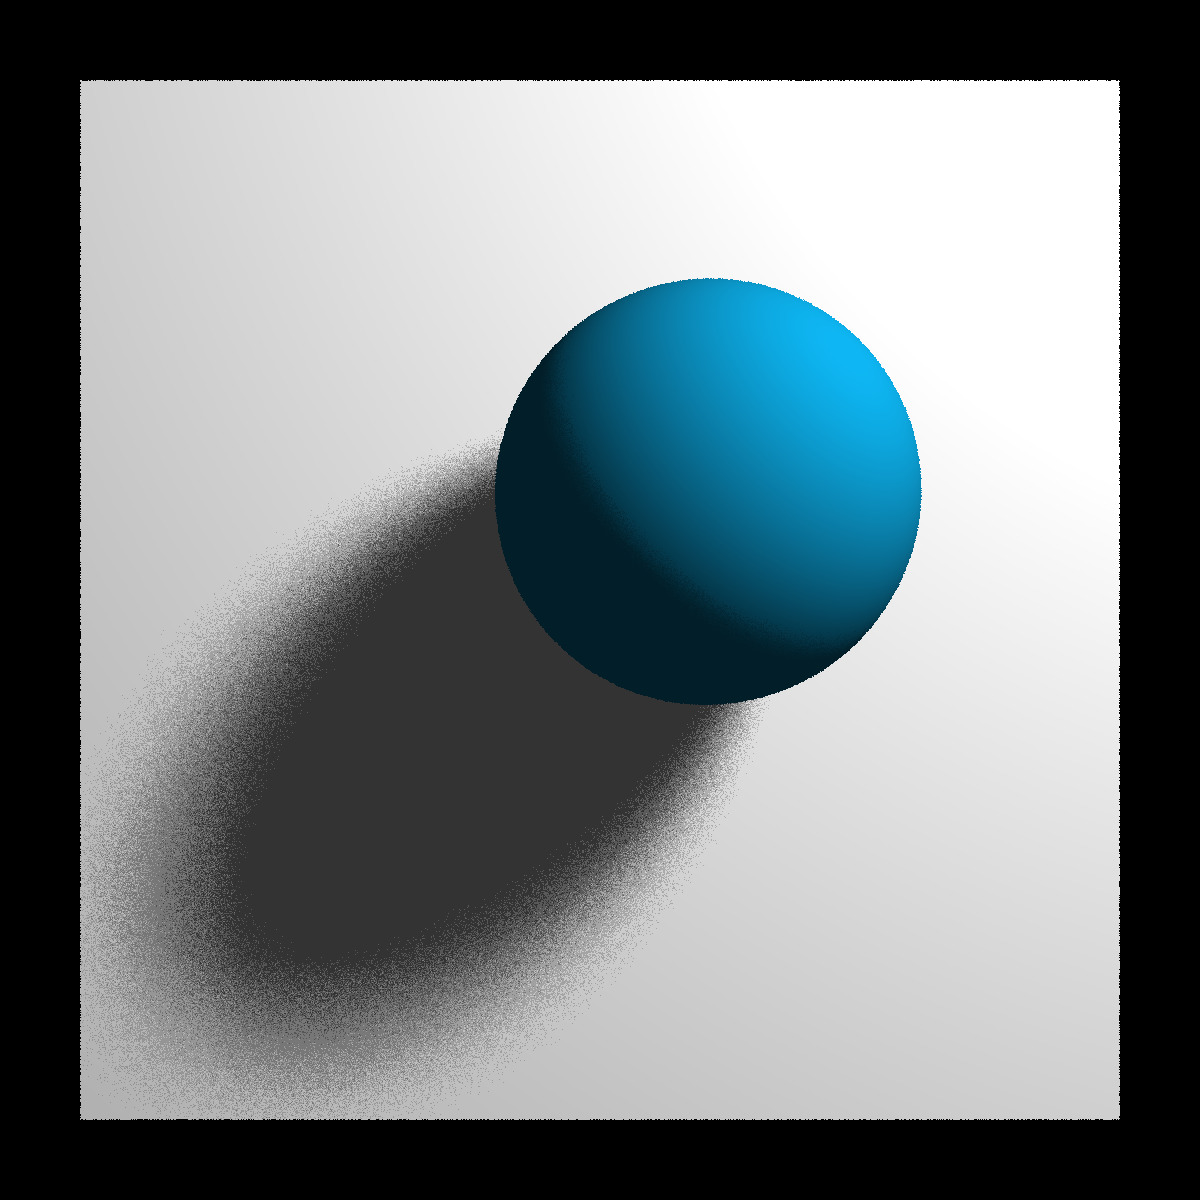
\includegraphics[width=4cm]{figures/shadow/shadow_rectangle_4_random.jpg}
    % \caption{Softer but noisy shadow. Area light with 4 randomly selected sample points}
    % \label{fig:shadowAreaLight4random}
  }
  \subfloat[Soft shadow without visible noise.\\Area light with 100 randomly selected sample points]{
    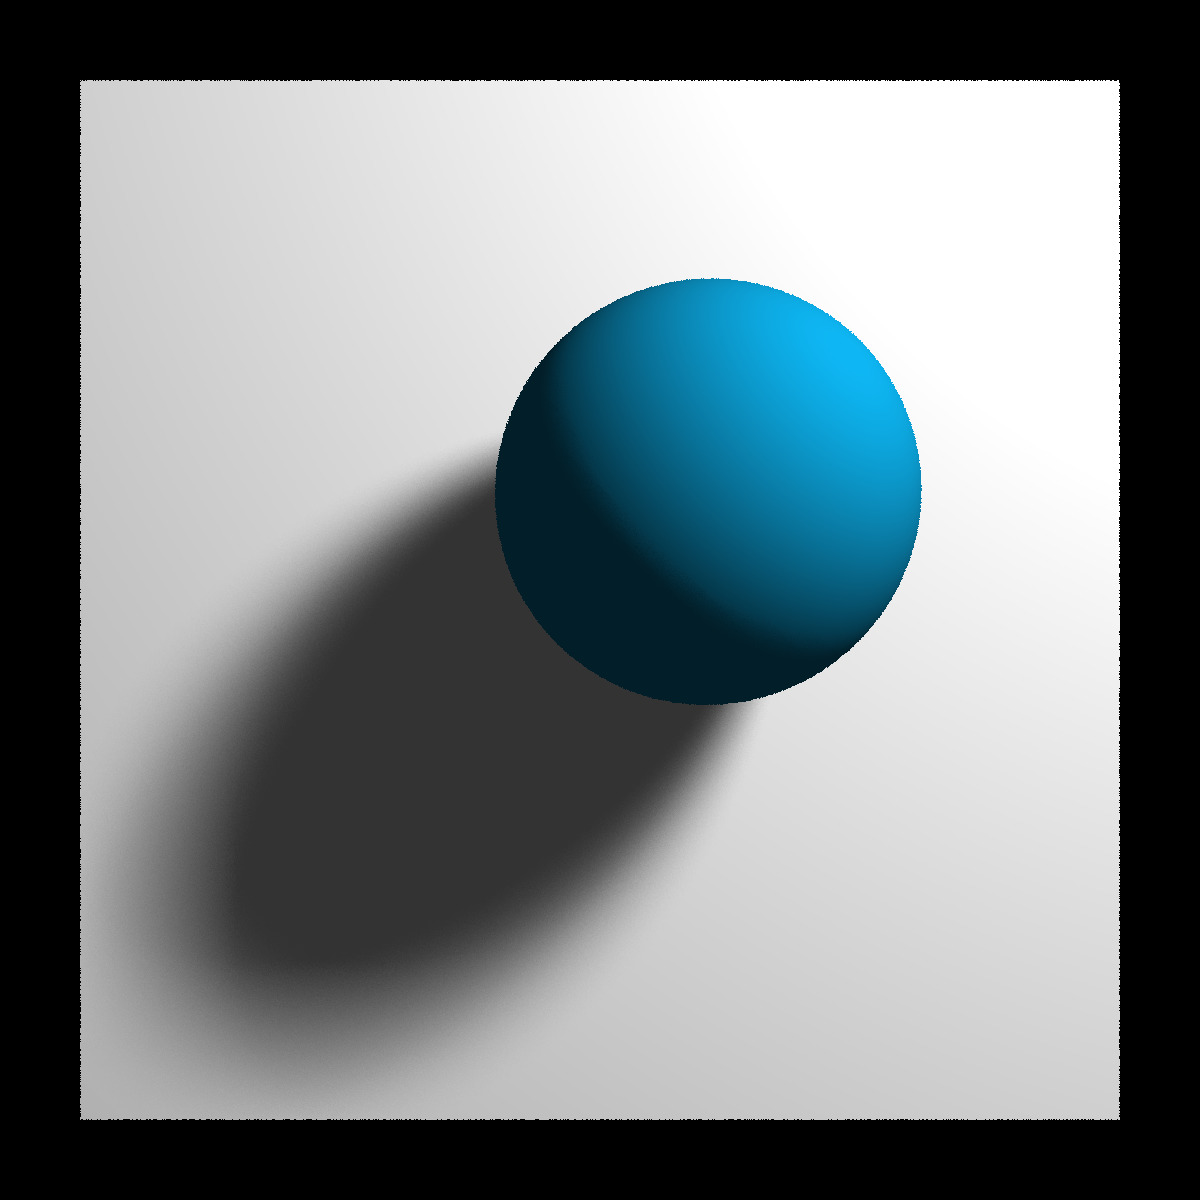
\includegraphics[width=4cm]{figures/shadow/shadow_rectangle_100_random.jpg}
    % \caption{Soft shadow without visible noise. Area light with 100 randomly selected sample points}
    % \label{fig:shadowAreaLight100random}
  }
  \caption{Comparison of different light sampling approaches}
  \label{fig:lightSampling}
  \end{figure}
%   \FloatBarrier

% \begin{figure}[h]
%   \centering
%   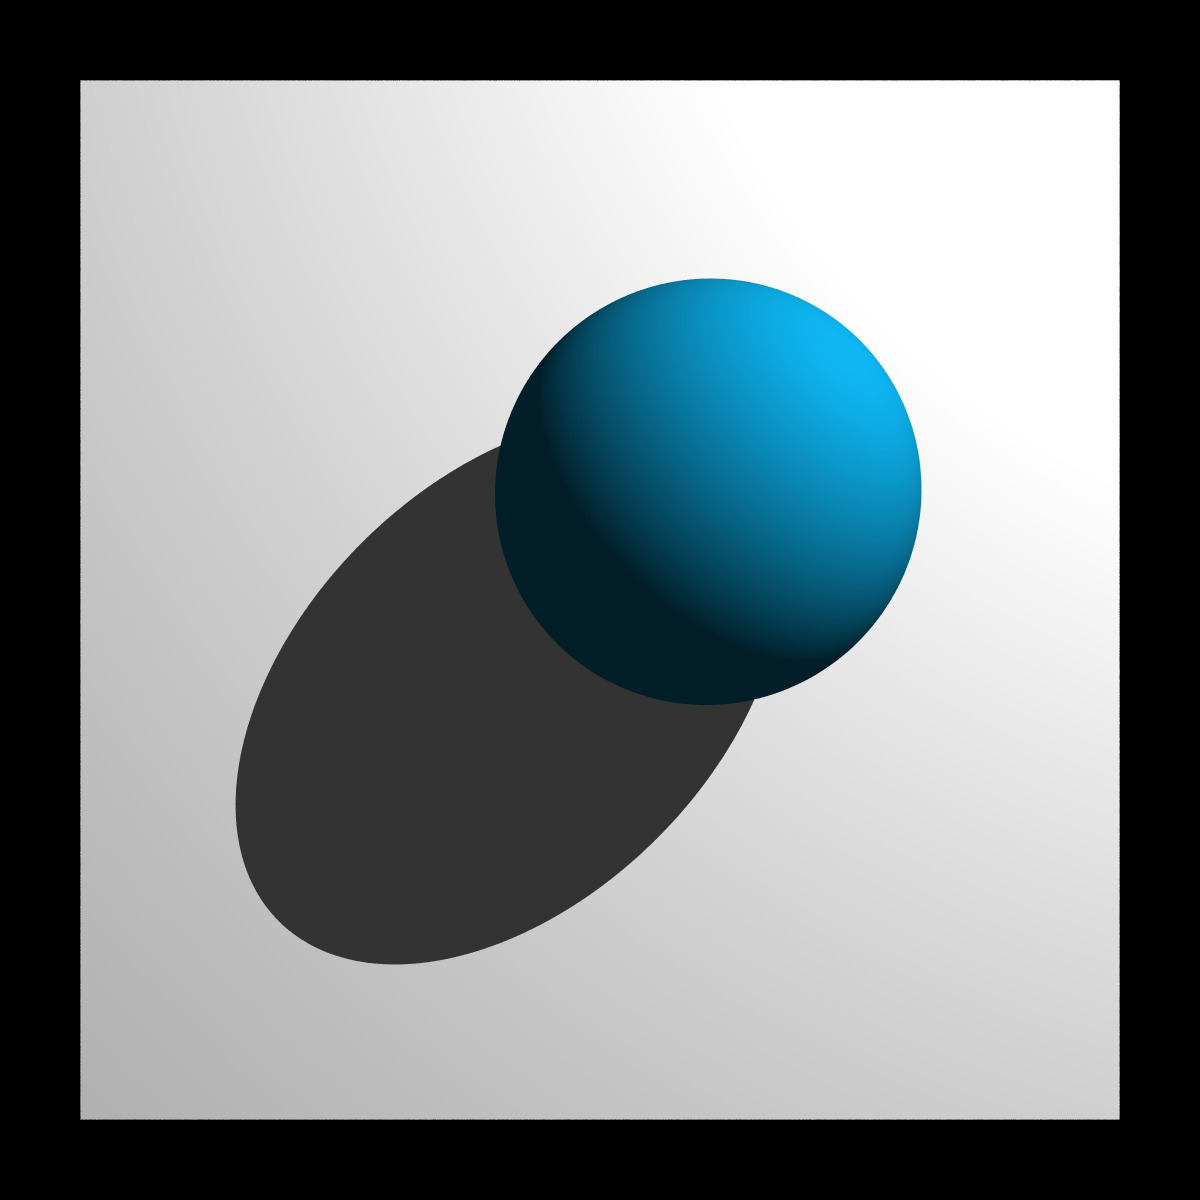
\includegraphics[width=5cm]{figures/shadow/shadow_pointlight.jpg}
%   \caption{Sharp shadow due to point light}
%   \label{fig:shadowPointLight}
% \end{figure}
% \begin{figure}[h]
%   \centering
%   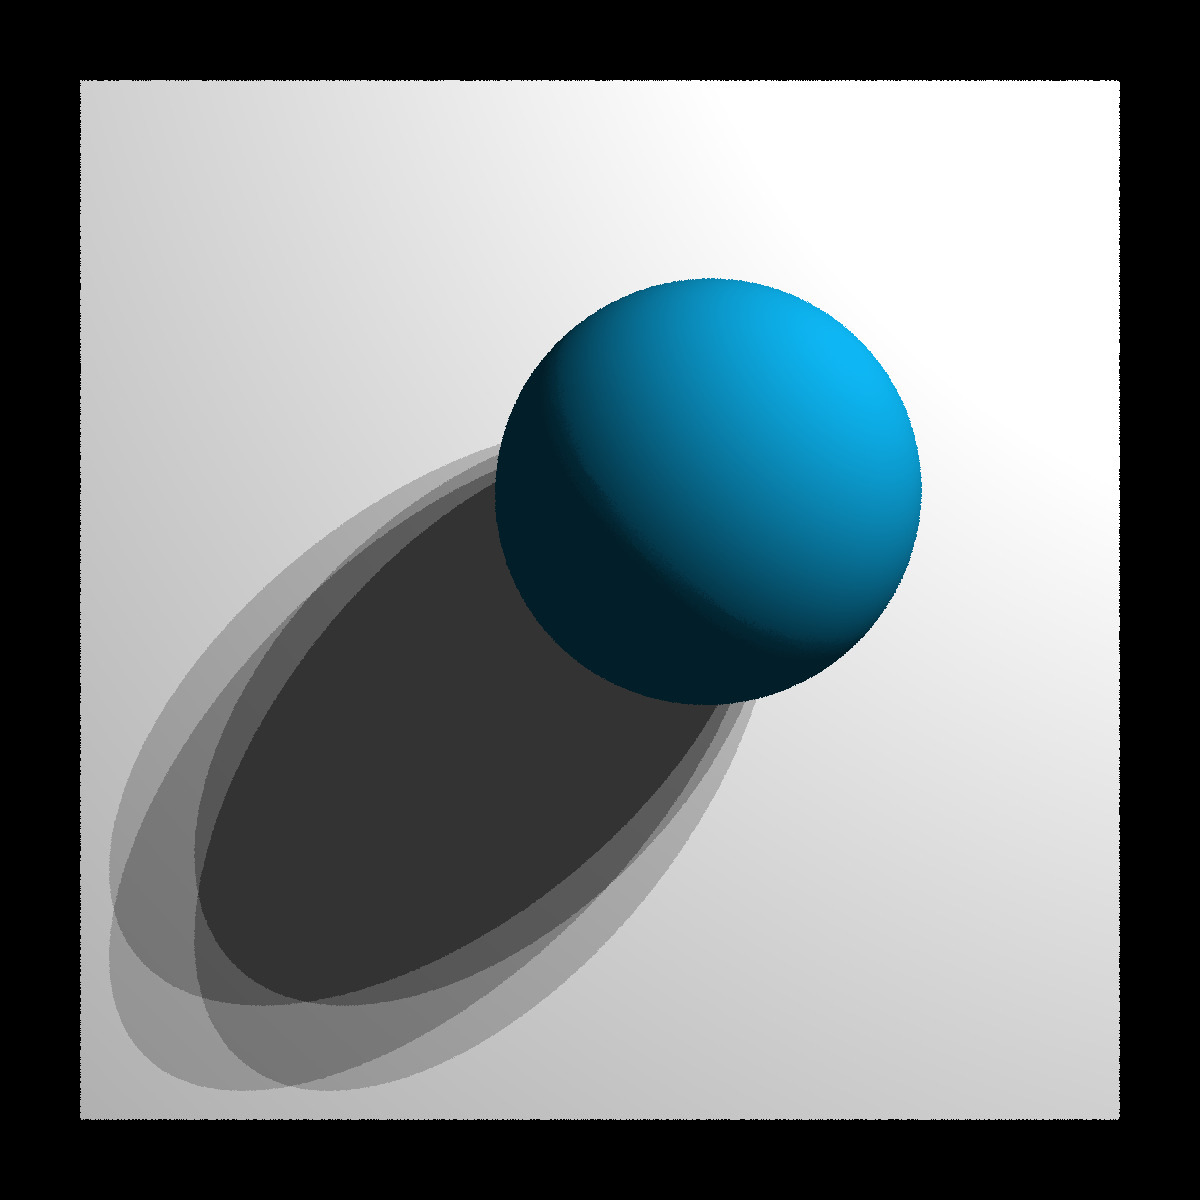
\includegraphics[width=5cm]{figures/shadow/shadow_rectangle_4_uniform.jpg}
%   \caption{Pattern in shadow. Area light with 4 uniformly selected sample points}
%   \label{fig:shadowAreaLight4uniform}
% \end{figure}
% \begin{figure}[h]
%   \centering
%   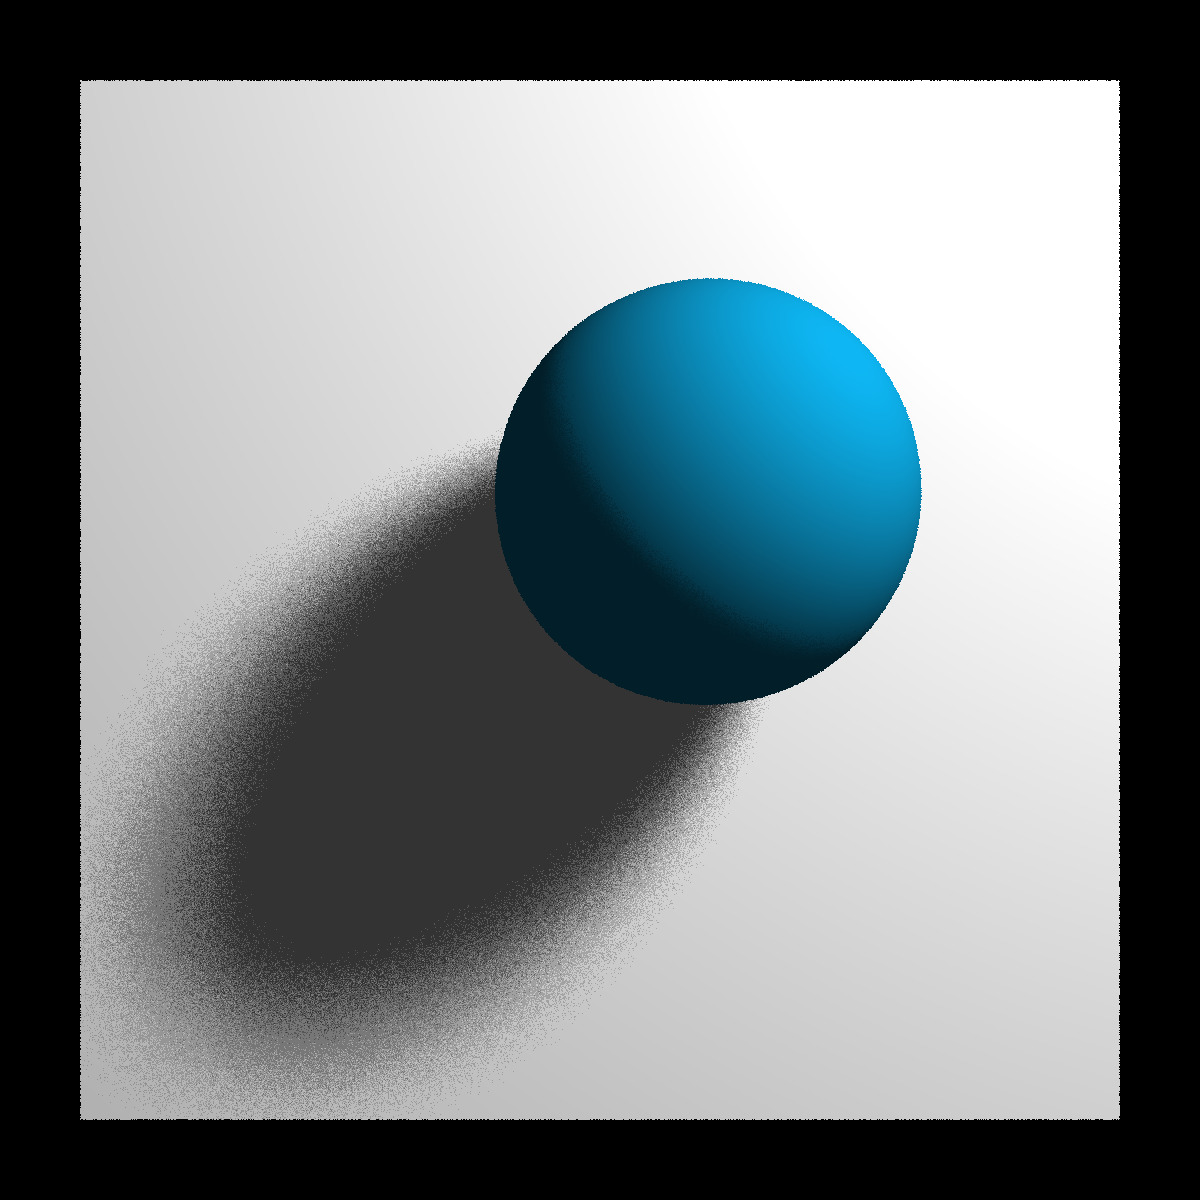
\includegraphics[width=5cm]{figures/shadow/shadow_rectangle_4_random.jpg}
%   \caption{Softer but noisy shadow. Area light with 4 randomly selected sample points}
%   \label{fig:shadowAreaLight4random}
% \end{figure}
% \begin{figure}[h]
%   \centering
%   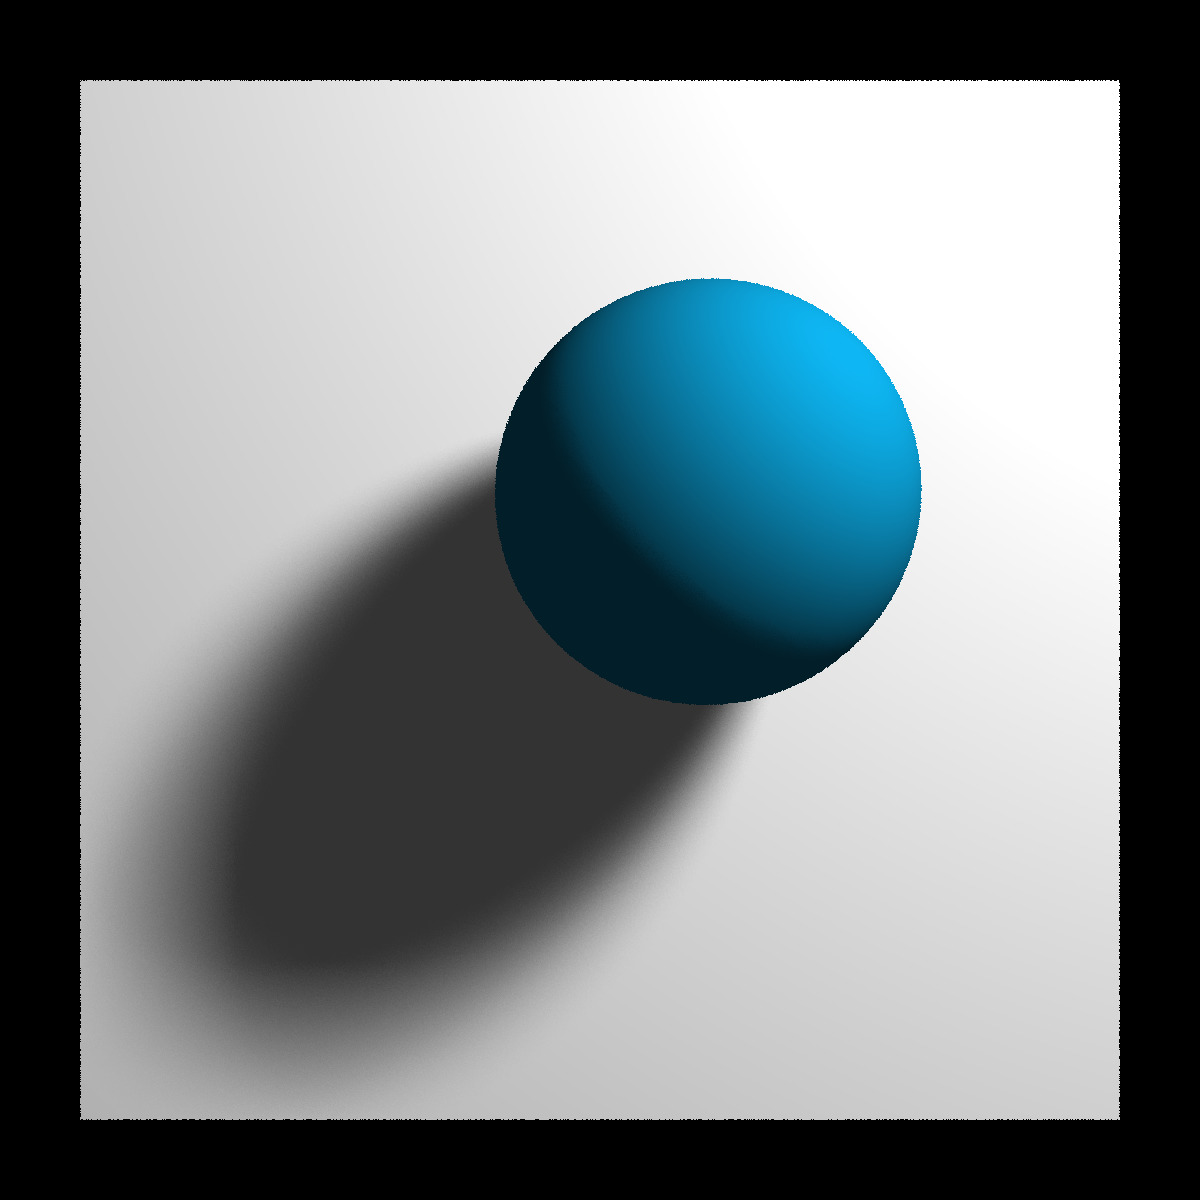
\includegraphics[width=5cm]{figures/shadow/shadow_rectangle_100_random.jpg}
%   \caption{Soft shadow without visible noise. Area light with 100 randomly selected sample points}
%   \label{fig:shadowAreaLight100random}
% \end{figure}

\subsection{Supersampling (anti-aliasing)}
The basic attempt to raytrace a scene is to shoot a primary ray starting from the camera through each pixel center. But this approach leads to 
pixelated edges in the scene as seen in Figure \ref{fig:super1}. 
To overcome this we can sample the scene in a much higher resolution by shooting more than one ray per pixel
and average those color results to determine the color of the pixel. Let N be the number of sub samples then the pixel color is calculates as follows.
\[pixelColor = \frac{1}{N}*\sum_{n=1}^{N}subPixelColor\] 
Figure \ref{fig:super16} uses 16 samples per pixel.

To subsample a pixel we use a jittered grid: we divide each pixel with a uniform grid and sample a random position in each grid cell.
% \begin{figure}[h]
%   \centering
%   
\includegraphics[width=5cm]{figures/supersampling/super1.jpg}
%   \caption{No super sampling: pixelated edge}
%   \label{fig:super1}
% \end{figure}
% \begin{figure}[h]
%   \centering
%   
\includegraphics[width=5cm]{figures/supersampling/super16.jpg}
%   \caption{16xsuper sampling: smoother edge }
%   \label{fig:super16}
% \end{figure}

\begin{figure}[ht]
  \centering
  \subfloat[No super sampling:\\pixelated edge]{
    
\includegraphics[width=4cm]{figures/supersampling/super1.jpg}
  }
  \subfloat[16xsuper sampling:\\smoother edge]{
    
\includegraphics[width=4cm]{figures/supersampling/super16.jpg}
  }

  \caption{Super sampling}
  \label{fig:lightSampling}
  \end{figure}


\section{Problems and accidental art}
The biggest challenge in this project was the correct calculation of the reflective and refractive rays using Snell's law and the Fresnel equations.
First of all dealing with the correct directions of incoming light and flipping the surface normal depending on if the intersection happens from outside or inside of the object.
And also using the correct equations for the calculations.

Also it was sometimes very challenging to assess the rendered scene in terms of correctness. Since the implemented technique does not take global illumination into
account it was sometimes hard to judge if the rendered scene is correct given the constrains of the algorithm. This was especially true for the glass sphere.

Errors in the code sometimes resulted in very nice, accidental art. Figure \ref{fig:art} shows the most beautiful accidents.

% \begin{figure}[h]
%   \centering
%   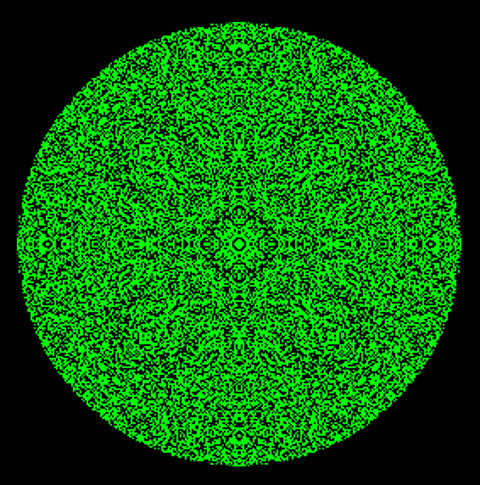
\includegraphics[width=5cm]{figures/art/art1.jpg}
%   \caption{Fractal pattern on sphere surface due to self occlusion}
%   \label{fig:art1}
% \end{figure}
% \begin{figure}[h]
%   \centering
%   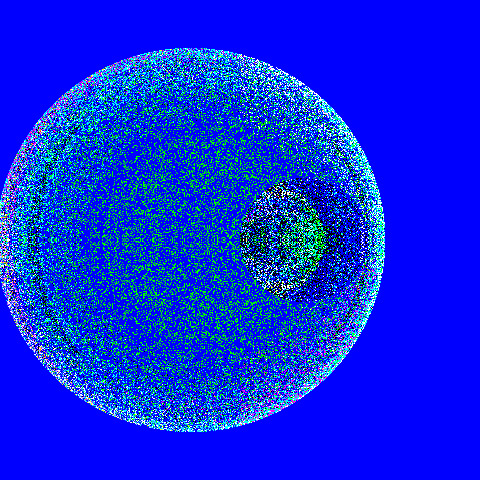
\includegraphics[width=5cm]{figures/art/art2.jpg}
%   \caption{Interesting looking death star formation what was supposed to be a smaller glass sphere in front of a bigger sphere}
%   \label{fig:art2}
% \end{figure}

\begin{figure}[ht]
  \centering
  \subfloat[Fractal pattern on sphere surface due to self occlusion]{
    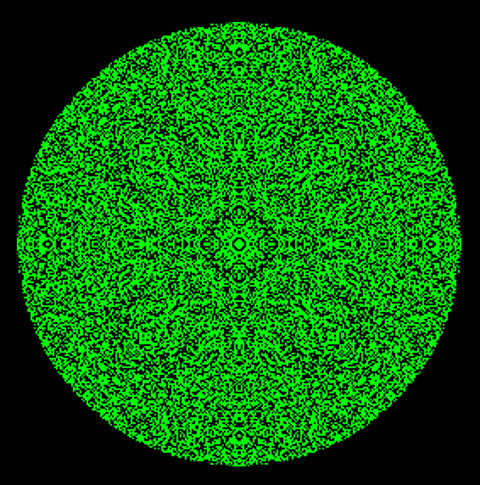
\includegraphics[width=4cm]{figures/art/art1.jpg}
  }
  \subfloat[Interesting looking death star formation what was supposed to be a smaller glass sphere in front of a bigger sphere]{
    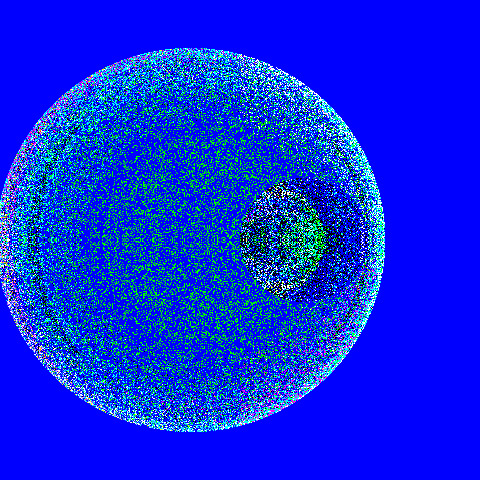
\includegraphics[width=4cm]{figures/art/art2.jpg}
  }

  \caption{Accidental art}
  \label{fig:art}
  \end{figure}


\section{Limitations and future work}
The biggest limitation of this implementation is the simulation of global illumination. By tracing the ray backwards from the eye into the scene
the algorithm assumes that only those rays that reach the eye contribute to the lighting of the scene. Lighting produced from reflection of light 
on surfaces are not taken into account. This is a large limitation in the attempt to render a realistic looking image.\\
Many different techniques exist to attempt to solve the rendering equation and produce a realistic looking image, 
e.g Photon Mapping, Path Tracing, Radiosity. In future work we want to implement and integrate one of those techniques into our project to overcome its limitations.





\clearpage

resources\\
https://en.wikipedia.org/wiki/Supersampling \\
https://en.wikipedia.org/wiki/UV_mapping#Finding_UV_on_a_sphere \\


% \clearpage

% \section{Citations}

% Some examples of references. A paginated journal article~\cite{Abril07}, an enumerated journal article~\cite{Cohen07}, a reference to an entire issue~\cite{JCohen96}, a monograph (whole book) ~\cite{Kosiur01}, a monograph/whole book in a series (see 2a in spec. document)~\cite{Harel79}, a divisible-book such as an anthology or compilation~\cite{Editor00} followed by the same example, however we only output the series if the volume number is given~\cite{Editor00a} (so Editor00a's series should NOT be present since it has no vol. no.), a chapter in a divisible book~\cite{Spector90}, a chapter in a divisible book in a series~\cite{Douglass98}, a multi-volume work as book~\cite{Knuth97}, an article in a proceedings (of a conference, symposium, workshop for example) (paginated proceedings article)~\cite{Andler79}, a proceedings article with all possible elements~\cite{Smith10}, an example of an enumerated proceedings article~\cite{VanGundy07}, an informally published work~\cite{Harel78}, a doctoral dissertation~\cite{Clarkson85}, a master's thesis~\cite{anisi03}, an finally two online documents or world wide web resources~\cite{Thornburg01, Ablamowicz07}.

% \begin{acks}
%  This work was supported by the [...] Research Fund of [...] (Number [...]). Additional funding was provided by [...] and [...]. We also thank [...] for contributing [...].
% \end{acks}

% %\clearpage

% \bibliographystyle{ACM-Reference-Format}
% \bibliography{sample}

\end{document}
\endinput
